% !TeX spellcheck = pt_BR
\documentclass[12pt,oneside,a4paper,article]{abntex2}

% ----------------------------------------------------------
% PACOTES
% ----------------------------------------------------------

% ---
% Pacotes fundamentais
% ---
%\usepackage{multicol}           
\usepackage{cmap}               % Mapear caracteres especiais no PDF
\usepackage[T1]{fontenc}        % seleção de códigos de fonte.
\usepackage[utf8]{inputenc}     % determina a codificação utiizada (conversão automática dos acentos)
\usepackage{makeidx}            % cria o indice
\usepackage{hyperref}           % controla a formação do índice
\usepackage{lastpage}           % usado por abntex2-fichacatalografica.tex
\usepackage{indentfirst}        % Identa o primeiro parágrafo de cada seção.
%\usepackage{nomencl}            % Lista de simbolos
\usepackage{graphicx}           % Pacote para inserir imagens JPEG/JPG e PNG
\usepackage{xcolor}             % Pacote de cores
\usepackage{graphicx,color}     % Pacote para definir cores diferentes para fonte

\newcolumntype{C}[1]{>{\centering\let\newline\\\arraybackslash\hspace{0pt}}m{#1}}

% ---
% Pacotes de citações
% ---
\usepackage[brazilian,hyperpageref]{backref}     % Paginas com as citações na bibl
\usepackage[alf]{abntex2cite}   % Citações padrão ABNT

% ---
% Alterações para melhor aparência do modelo article
% ---
% Elimina a marcação de capítulo nas seções e permite não se utilizar \chapter{}
\renewcommand{\thesection}{\arabic{section}}
% Altera o tamanho da fonte para Referências, com o tamanho de seção, já que não são usados capítulos.
\renewcommand{\ABNTEXchapterfontsize}{\Large}
% ---


% Title Page
\title{Make.a.List\\Análise de Requisitos}

\author{João Pedro Santos de Moura\\
		Marcus Vinicius Nunes Calisto\\
		Oto Braz Assunção}

\local{Departamento de Computação e Sistemas\\
	   Instituto de Ciências Exatas e Aplicadas\\
	   Universidade Federal de Ouro Preto}
	
\date{20 de novembro de 2015}


\begin{document}
\maketitle

\pagebreak

\tableofcontents

\pagebreak

\listoffigures

\pagebreak

\listoftables

\part{Introdução}
\section{Uma Breve Introdução}
	É comum que professores lecionem mais de um disciplina durante os períodos acadêmicos.
	Durante o período acadêmico, como parte da distribuição de créditos, é comum que os docentes reservem uma parte dos mesmos para resolução de listas de exercícios.

	Dependendo da disciplina, o processo de confecção e resolução destas listas pode se tornar custoso em relação ao tempo, pois a ementa da disciplina pode ser extensa e isso pode levar o professor a gastar muito tempo selecionando questões de acordo com a disciplina e seus tópicos.

\part{Descrição do Problema}
	\section{Descrevendo o Problema}
		\subsection{O Problema dos Professores}
			Tendo em vista que professores tendem a ministrar mais de uma turma, muitas vezes de diferentes disciplinas, o processo criativo de listas de exercícios pode se tornar extenuante nesses casos.
		
		\subsection{O Problema dos Alunos}
			Ao receber uma lista, é comum o aluno resolvê-la e esperar uma possível correção por parte do professor, seja durante uma aula específica ou agendando um horário.
			O problema é o tempo que isso custa ao aluno, que poderia ter acesso as respostas logo após fazer o exercício ou a partir de uma determinada semana definida pelo
			professor. Assim, o aluno seria capaz de conferir suas respostas sem tomar também o tempo do professor e o horário da aula seria usado para sanar as dúvidas
			mais relevantes.
			
\part{Objetivo}
	\section{O Objetivo}
		O objetivo geral é facilitar o processo de criação e correção de listas de exercício tanto para alunos quanto para professores.
		\subsection{Visando os Professores}
			O objetivo da aplicação é agilizar o processo de confecção de listas de exercícios por parte dos professores, além de poupar tempo com atendimento aos alunos
			que buscam respostas de tais questões presentes nessas listas.

		\subsection{Visando os Alunos}
			Evitar que o aluno perca muito tempo para consultar o professor com relação à respostas de exercícios e seja capaz de conferir por si próprio se sua resolução de
			uma determinada questão está certa ou não.
			
\part{Escopo da Aplicação}
	\section{O Escopo}
		O ambiente acadêmico será o escopo da aplicação mas nada impede que uma empresa possa adaptar o sistema de forma a gerar essas listas como  testes em cursos de
		treinamentos mas para esta aplicação em específico, o espoco é o ambiente acadêmico, que é onde mais se usa esse tipo ferramenta.

\part{Descrição do Produto}
	\section{Descrevendo o Produto}
		
		\subsection{A Web}
			Dar o contexto da web
		
		\subsection{A aplicação}
			Usar o contexto para mostrar porque é importante que ela seja desenvolvida nessa plataforma, o seu objetivo, funcionamento, para quem e porquê eles devem usar.
\part{Caso de Uso}
	\section{Casos de Uso}
		Nesta seção são apresentados os artefatos correspondentes aos casos de uso do produto, bem como os seus respectivos diagramas.
		
		\subsection{Caso de Uso I - Adicionar Disciplina}
	
		\subsection{Caso de Uso II - Adicionar Tópico}
	
		\subsection{Caso de Uso III - Adicionar Questão}
	
		\subsection{Caso de Uso IV - Gerar Lista como Professor}
	
		\subsection{Caso de Uso V - Gerar lista como Aluno}
	
		\subsection{Caso de Uso VI - Recuperar uma Lista Gerada}

\part{Classes}
	\section{Classes}
		Nesta seção são apresentadas as classes que integram a aplicação, bem como um diagrama para cada e um diagrama de classes onde mostra
		as relações entre elas.
		
		\subsection{Usuário}
			Classe genérica para compartilhar atributos em comum entre as subclasses Administrador, Professor e Aluno.
	
				\subsubsection{Administrador}
					Usuário capaz de inserir, remover e atualizar outros usuários Professores e Alunos bem como adicionar, editar e remover todas as categorias do
					sistema. Tem todos os privilégios do sistema.
				\subsubsection{Professor}
				Usuário capaz de inserir e remover disciplinas, tópicos e questões.
	
				\subsubsection{Aluno}
					Usuário com o menor nível de privilégio, capaz de recuperar a lista de acordo com um código único e visualizar as respostas depois de uma data definida
					por quem gerou a lista.

		\subsection{Disciplina}
			A classe Disciplina é responsável por agrupar questões de uma determinada área, para que o professor seja capaz de gerar essa lista de forma aleatória que seja condizente
			com a área da disciplina.
	
		\subsection{Tópico}
			Referencia a um tópico específico de uma determinada disciplina, por exemplo, alocação dinâmica de memória é um tópico da disciplina Programação.
	
		\subsection{Questão}
			Está relacionada a uma disciplina e um tema e contém a pergunta e sua resposta.
	
		\subsection{Lista}
			Uma coleções de questões. Possui um ID e uma coleção de questões.
		
		\subsection{Diagrama de Classes}
			\begin{figure}[h]
				\centering
				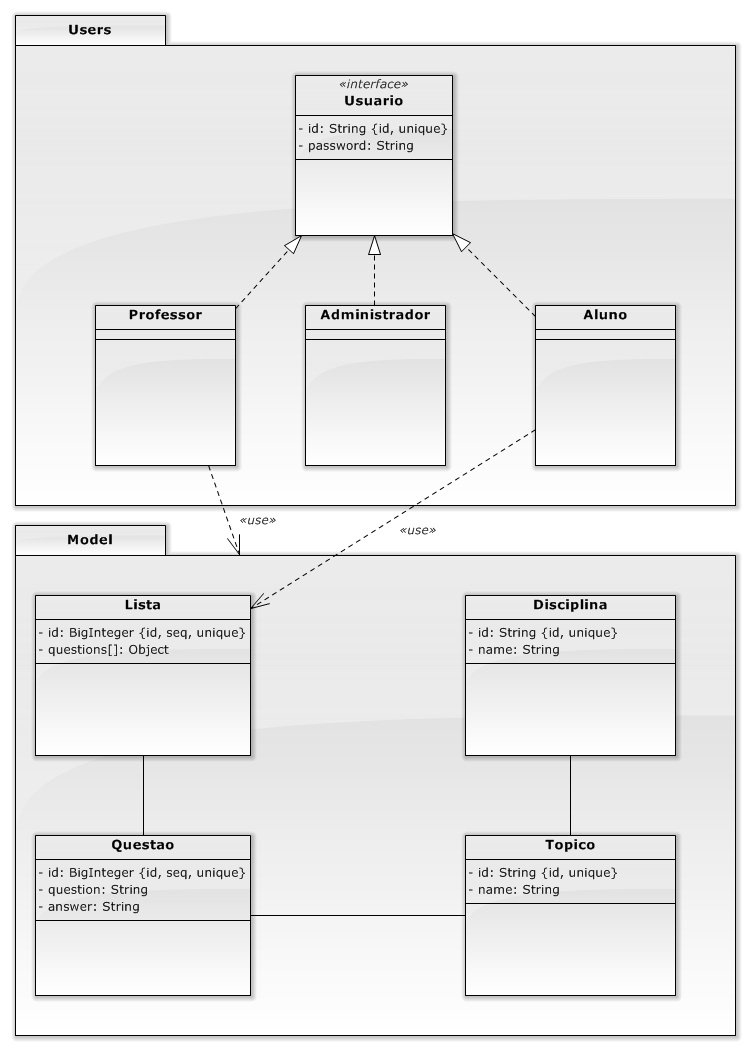
\includegraphics[scale=.5]{Imagens/DiagramaDeClasses}
				\caption{Diagrama de classes}
				\label{fig:diagramaclasses}
			\end{figure}
		
		\subsection{Diagrama de Pacotes}
		\begin{figure}[h]
			\centering
			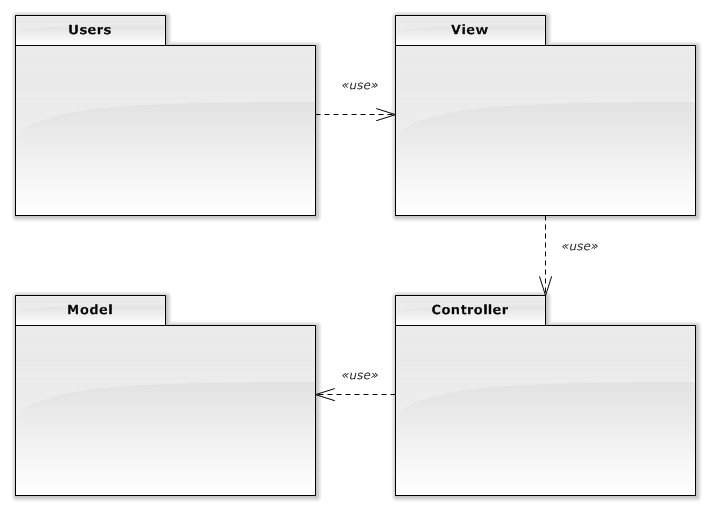
\includegraphics[scale=.7]{Imagens/DiagramaDePacotes}
			\caption{Diagrama de pacotes}
			\label{fig:diagramapacotes}
		\end{figure}
			

\part{Banco de Dados}
	\section{O Banco de Dados}
		O banco de dados da aplicação será o MySQL, que está incluído na solução Laragon\footnote{URL DO LARAGON} para a plataforma Windows e possui versões tanto para Mac quanto distribuições Linux. Outro motivo que levou a escolha da tecnologia foi por ser de código aberto, com amplo suporte da comunidade.
		
		\subsection{Diagrama Entidade-Relacionamento}
			\begin{figure}[h]
				\centering
				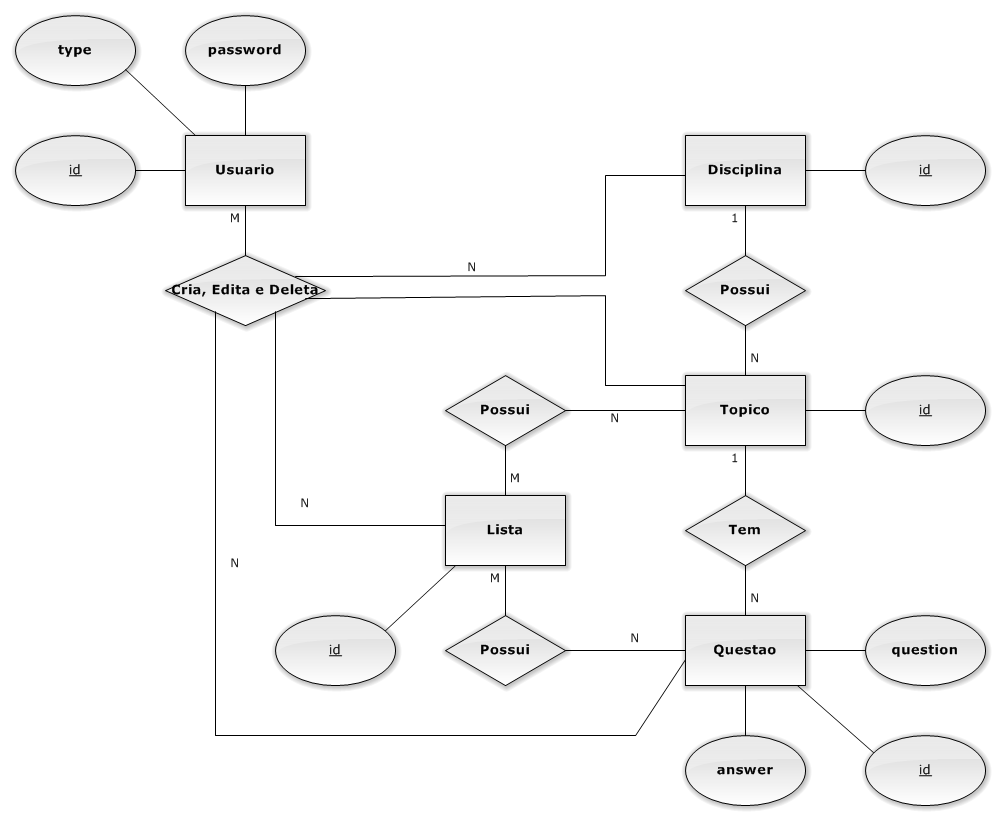
\includegraphics[scale=.6]{Imagens/Entidaderelacionamento}
				\caption{Diagrama Entidade-Relacionamento do banco de dados da aplicação}
				\label{fig:Entidaderelacionamento}
			\end{figure}

	
		\subsection{Diagrama Relacional}
	

\part{Protótipos}
	\section{Prototipação}
		Nesta seção são apresentados os protótipos para cada interação e casos de uso apresentados anteriormente.
		
		\subsection{O Laravel}
			Como requisito do projeto, essa solução será desenvolvida usando um \textit{framework} que tem como base o padrão \textit{Model-View-Controller}, ou MVC.
			Devida a experiência dos integrantes da equipe, será usado o Laravel\footnote{Disponível em: \url{http://laravel.com/}. Acesso em 16 de novembro de 2015.}
	
		\subsection{Tela de Login}
	
		\subsection{Telas do Professor}
			\subsubsection{Adicionar Disciplina}
			\subsubsection{Adicionar Tópico}
			\subsubsection{Adicionar Questão}
			\subsubsection{Geração de Listas}
		
		\subsection{Tela do Aluno}
		

\part{Cronograma}

\part*{Anexos}

% Refeências

\end{document}          
